\documentclass[12pt,english]{article}
\usepackage[T1]{fontenc}
\usepackage{mathptmx}
%\renewcommand{\familydefault}{\sfdefault}
\usepackage[latin9]{inputenc}
\usepackage{multirow}
\usepackage{multicol}
\usepackage[letterpaper]{geometry}
\geometry{verbose,tmargin=2cm,bmargin=2cm}
\usepackage{float}
\usepackage{amstext}
\usepackage{amsmath}
\usepackage{mathptmx}
\usepackage{amsthm}
\newtheorem{hypothesis}{Hypothesis}
\usepackage{multirow}
\newtheorem{result}{Result}
%\usepackage{theorem}
%\newtheorem{hypo}{Hypothesis}
\usepackage{harvard}
\usepackage[font=small,labelfont=bf]{caption}
\usepackage{graphicx}
\usepackage{subfig}
\usepackage{url}
\usepackage{indentfirst}
%\graphicspath{{Figures/}}
\usepackage{amsmath}
\usepackage{setspace}
\usepackage{esint}
\onehalfspacing
\usepackage{babel}
\usepackage{indentfirst}
\doublespacing 

\begin{document}

\title{Endogenous Timing in the Conflict Games}

\author{Youngseok Park\footnotemark[] \thanks{Corresponding Author. \textit{Email:}
    ypark@colby.edu \textit{Address:} 
Department of Economics, Colby College, Waterville, ME 04901. We thank Tomas Sj\"ostr\"om, Larry Samuelson, Kyung Hwan Baik, and many seminar participants at the Maine Economics conference 2018, the New England Experimental Economics Workshop 2018, and the 29th Stony Brook International Conference on Game Theory 2018.}
 \and Jean Paul Rabanal \thanks{Department of Banking and Finance, Monash University.}}
\date{\today}
\maketitle

\begin{abstract}
\noindent This paper investigates endogenous timing in the conflict games of Baliga and Sj\"ostr\"om (2012 [B]). If the game has strategic complements, then a dovish player always moves early while a hawkish player always delays. Consequently, endogenous timing increase the likelihood of a peaceful outcome. If the game has strategic substitutes, then all players choose the first period and the game will be always a simultaneous-move game. 
\end{abstract} 

\textit{JEL Classification}: D74, D82 \par 
\textit{Keywords}: Conflict; Endogenous timing; Global games

\newpage
\section{Introduction}

%The fear about the counterparty's hawkishness in the conflict games of Baliga and Sj\"ostr\"om triggers belligerent behavior.  Even if players are not intrinsically hawkish, they may opt for an aggressive action, because they are unable to rule out the possibility that the opponent is hawkish, or that the opponent thinks that they are hawkish (Baliga and Sj\"ostr\"om, 2009). Thus, their model captures one of the explanations present in Hobbes (1651) of why parties are trapped in a state of war (Baliga and Sj\"ostr\"om, 2012 [A]). \par 
The strategy of conflict may involve strategic timing of move because an early action or absence of early action can be a clue to find the opponent's type. In the literature on conflict games (Baliga and Sj\"ostr\"om, 2004, 2009, 2012 [A], [B]; Jackson and Morrelli, 2011), the order of play is exogenously given, mostly by a simultaneous move. However, this assumption is quite restrictive because in many real-world situations of conflict, a party can choose whether to move early or late.  How does a player choose timing of move and what can be shown in the conflict games by endogenous timing? \par
In our extended conflict game with endogenous timing, we find that state of war appears less often than the simultaneous-move conflict game in Baliga and Sj\"ostr\"om (2012 [B]) if the game has strategic complements. Theory predicts that a dovish player moves early while a hawkish leader delays in order to observe the counterparty's action. That is, the order of play serves as a coordination device that helps avoiding a conflict.\par 
This result echos the early attempts of reconciliation by the South Korean leader followed suit by the actions of the hawkish North Korean leader.\footnote{For details on this conflict, see Buzo (2002) and Cummings (2005).}  It also capture Schelling's insights on coordination and conflict: Some focal point for a concerted choice, some clue to coordination, and some rationale for the convergence of the participants' mutual expectations might be a potent force not only in pure coordination but in the mixed situation that includes conflict (Schelling, 1960).\par  %Furthermore, the results remind us of Jervis' insights on cooperation under the security dilemma: Anything that increases each side's expectation that the other will cooperate may make cooperation more likely (Jervis, 1978). \par %Interestingly, our results are robust to the presence of an extremist third-party who seeks to alter the peaceful outcome. \par%For the North's leader, a wait-and-see attitude may be a best response, given the low cost of tension with the South and the uncertainty regarding the stand of the South's new regime. For the South's leader, early dovish moves may be a dominant strategy due to the high cost of tension and the belief that the North will reciprocate.
%In the simultaneous-move conflict games, players choose a dovish action or a costly hawkish action. The cost of the hawkish action is private information, so is ``type'' of the players. The private cost can be interpreted as the cost of building weapons or the welfare loss for being hawkish. Players that have extremely low cost are dominant strategy hawks while players with extremely high cost are dominant strategy doves. Then, there exists a cutoff strategy in which the players with lower cost than the cutoff will behave aggressively (Baliga and Sj\"ostr\"om, 2012 [B]). Following Baliga and Sj\"ostr\"om (2012 [B]), we denote the types around the cutoff as ``coordination types,'' because they will act dovish if the other player reciprocates. \par 
%In the extended games with endogenous timing, the presence of the coordination types encourages some players to move first resolving the state of war. With strategic complements, a player moves early if she plans to be dovish. Thus, the dovish types move early, and play the dovish action. Dominant strategy hawks delay and act aggressively regardless of the counterparty's choice. The coordination types have a wait-and-see attitude. They are unwilling to commit too early, but if the opponent plays the dovish action, then they will follow suit. These results capture Schelling's insights on coordination and conflict: Some focal point for a concerted choice, some clue to coordination, and some rationale for the convergence of the participants' mutual expectations might be a potent force not only in pure coordination but in the mixed situation that includes conflict (Schelling, 1960). Furthermore, the results remind us of Jervis' insights on cooperation under the security dilemma: Anything that increases each side's expectation that the other will cooperate may make cooperation more likely (Jervis, 1978). \par 
If the game has strategic substitutes, coordination does not occur. The first movers have an upper hand which incentives all players to move first, leading to a simultaneous interaction previously studied in Baliga and Sj\"ostr\"om (2012 [B]).\par  %In that environment, players follow a cutoff strategy according to their type.\par %Moreover, Baliga and Sj\"ostr\"om (2012) show that a third-party can strategically manipulate the conflict. \par
Endogenous timing has been extensively studied in other contexts such as duopoly games (e.g. Hamilton and Slutsky, 1990; Maliath, 1993; Normann, 2002), contest games (e.g. Baik and Shogren, 1992), under pure information externalities (e.g. Chamley and Gale, 1994; Gul and Lundholm, 1995), coordination games (e.g. Bolton and Farrell, 1990; Brindisi et al., 2014; Dasgupta, 2007; Farrell, 1987). Specifically, our results are similar to Brindisi et al. (2014). In their pure coordination game, players decide to invest in a joint project whose return is uncertain. They find that the player with high beliefs about the return invests early, and thereby facilitates coordination to undertake the project. \par
We begin in Section 2 with a description of the strategy in conflict games and present the sequential-move game. We examine the extended game with endogenous timing in Section 3. We conclude in Section 4.\par 

\section{The Strategy in the Conflict Games}
Consider the two-player conflict game of Baliga and Sj\"ostr\"om (2012 [B]). Two players $A$ and $B$ simultaneously choose either a hawkish action $H$ or a dovish action $D$. The payoff for player $i \in \{A,B\}$ is described in Table \ref{t:payoff}, where the row (column) represents the player $A$'s ($B$'s) choice.

\begin{center}
\begin{table}[h!]
\centering
\begin{tabular}{ccc}
  & $H$  & $D$  \\
$H$ & $-c_A, -c_B$ & $\mu-c_A, \mu-c_B$ \\
$D$ & $-d,-d$ & $0,0$ 
\end{tabular}   
\caption{The conflict game} 
\label{t:payoff}
\end{table}
\end{center}\par

In Table \ref{t:payoff}, $d>0$ is the cost of being caught out by playing $D$ when the opponent plays $H$. $\mu>0$ represents a benefit from being more hawkish than the opponent. Player $i$ has an idiosyncratic private cost $c_i$ of taking the hawkish action $H$, referred to as her type. Interpretations of $c_i$ may be privately known costs of building weapons or welfare loss for being hawkish. Player $i$'s type is independently drawn from the same distribution, $F$, which is a continuous cumulative distribution function with support $[\underline{c}, \bar{c}]$, and where $F^{\prime}(\cdot)>0$. The family of player $i$'s type is described in Figure \ref{fig:1}.\par
\begin{figure}[h]
\centering
	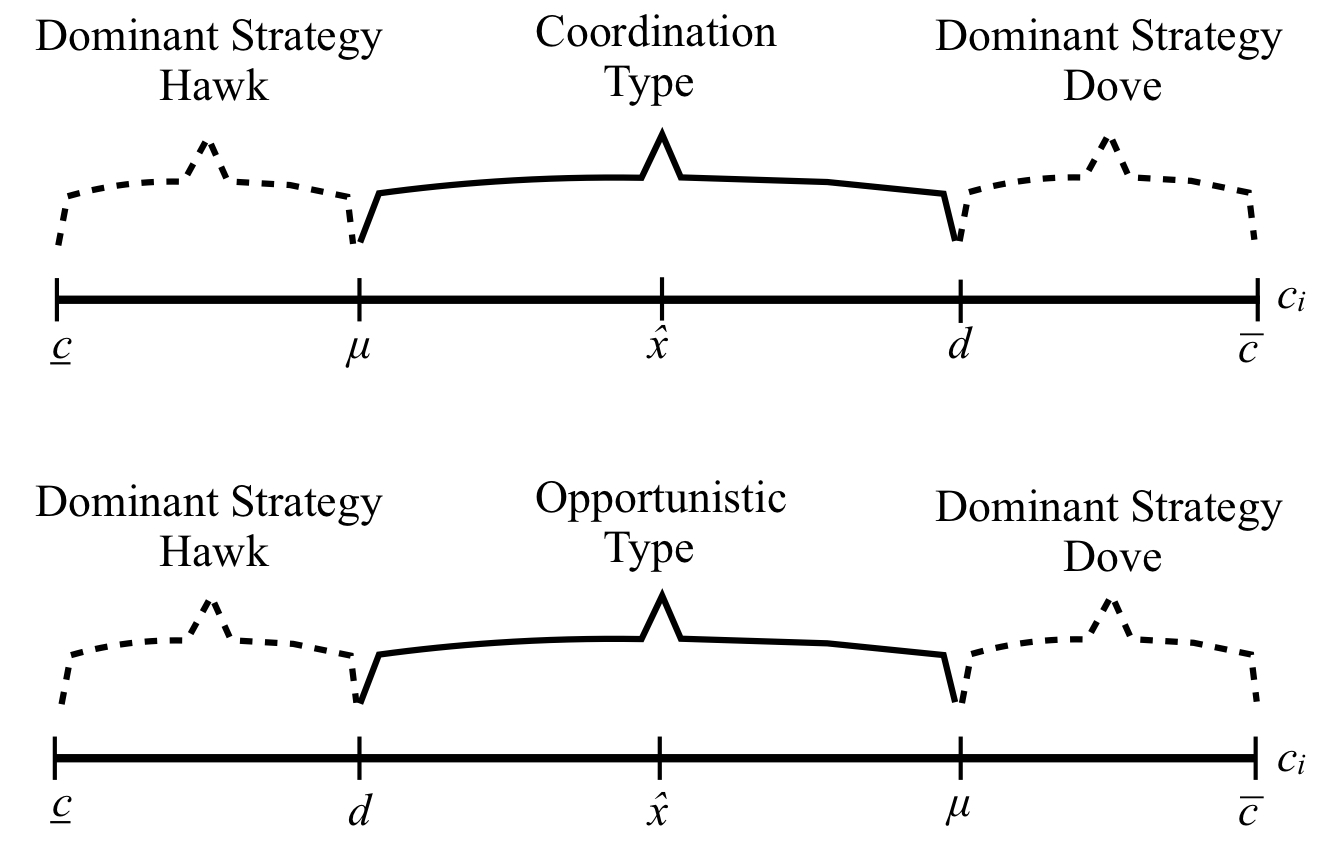
\includegraphics[scale=0.24]{figure1.jpg}
	\caption{The family of types under strategic complements (top) and substitutes (bottom)}
	\label{fig:1}
\end{figure}
Notice that the game has strategic complements ---the players are coordination types unless they are dominant strategy types--- if $d>\mu$; and the game has strategic substitutes ---the players are opportunistic types unless they are dominant strategy types--- if $\mu> d$. \par

Since player $i$'s expected net payoff from playing $H$ instead of $D$ is monotone in $c_i$, all Bayesian Nash equilibrium (BNE) must be in a cutoff strategy, in which player $i$ has a cutoff point $x \in [\underline{c}, \bar{c}]$, where she plays $H$ if and only if $c_i \leq \hat{x}$ (see Figure \ref{fig:1}). Specifically, player $i$'s best response to player $j$'s cutoff $x_j$ is the cutoff
\begin{equation}
    x_i=\Gamma(x_j)\equiv \mu+(d-\mu)F(x_j),
    \label{eq:xhat}
\end{equation}
\noindent where the function $\Gamma(\cdot)$ is the best response function for cutoff strategies, and $F(x_j)$ is the probability that player $j$ plays $H$. Lemma 1 states Baliga and Sj\"ostr\"om's (2012 [B]) result for the simultaneous-move conflict game.
\newtheorem{lem}{Lemma}
\begin{lem}
In the unique Bayesian Nash equilibrium (BNE), the probability player $i$ plays $H$ is $F(\hat{x})$, where $\hat{x}$ is the unique fixed point of $\Gamma(x)$  $ \in [\underline{c}, \bar{c}]$, in equation (\ref{eq:xhat}).
\end{lem}\par
In the BNE, player $i \in \{A,B\}$ uses the cutoff strategy where they play $H$ if $c_i \leq \hat{x}$. Even if player $i$ is not intrinsically hawkish (i.e., non-dominant strategy hawk, $\mu<c_i \leq \hat{x}$), she ends up being hawkish because she cannot rule out the possibility that the opponent is extremely hawkish, or that the opponent thinks that she is extremely hawkish. This reasoning causes spirals of fear, which lead to the unique BNE where players $A$ and $B$ may end up being in a state of war. Baliga and Sj\"ostr\"om (2012 [A]) capture this reasoning and define it as ``the Hobbesian trap.''\par
Before we present the game with endogenous timing, we set the stage by describing the perfect Bayesian equilibrium (PBE) of the sequential-move conflict games. 

\subsection{The Sequential-Move Conflict Games }
We examine the sequential-move conflict games where player $i$ is the first mover and player $j \neq i$ is the second mover. Lemma 2 states the unique PBE of the sequential-move conflict games.
\begin{lem}
There exists a unique perfect Bayesian equilibrium (PBE) where the first mover uses the cutoff strategy, $\sigma_i(c_i)=H$ if $c_i\leq \bar{x} \equiv F(\mu)d+\mu(1-F(d))$. $\bar{x}<\hat{x}$ when the game has strategic complements, and $\hat{x}<\bar{x}$ when the game has strategic substitutes.
\end{lem}
\begin{proof}
See Appendix.
\end{proof} \par 
%When the game has strategic complements ($d>\mu$), if the first mover player $i$ plays $D$, then the second mover player $j$ will play $D$ unless player $j$ is a dominant strategy hawk. That is, if player $i$ plays $D$ first, then player $j$ will be more likely to play $D$, compared to the simultaneous-move game. To see this, the probability of playing $D$ is $1-F(\mu)$ in the sequential-move game, whereas it is $1-F(\hat{x})$ in the simultaneous-move game. Hence, the cutoff point for the first mover, player $i$, in the sequential-move game, labelled as $\bar{x}$, will be smaller than the cutoff point in the simultaneous-move game, $\hat{x}$.\par
To illustrate the unique PBE when the game has strategic complements, player $j$ plays $D$ if player $i$ chooses $D$, unless player $j$ is a dominant strategy hawk. Player $j$ plays $H$ if player $i$ chooses $H$, unless player $j$ is a dominant strategy dove. Given player $j$'s strategy, player $i$ plays $H$ if the expected payoff of playing $H$ is greater than the expected payoff of playing $D$.\par
%When the game has strategic substitutes ($\mu>d$), if the first mover player $i$ plays $D$, then the second mover player $j$ will play $H$ unless player $j$ is a dominant strategy dove. That is, if player $i$ plays $D$ first, then player $j$ will be less likely to play $D$, compared to the simultaneous-move game. To see this, the probability of playing $D$ is $1-F(d)$ in the sequential-move game, whereas it is $1-F(\hat{x})$ in the simultaneous-move game. Hence, the cutoff point to play $H$ for the first mover player $i$  in the sequential-move game ($\bar{x}$) is larger than the cutoff point in the simultaneous-move game ($\hat{x}$).\par
To illustrate the unique PBE when the game has strategic substitutes, player $j$ plays $D$ if player $i$ chooses $H$, unless player $j$ is a dominant strategy hawk. Player $j$ plays $H$ if player $i$ chooses $D$, unless player $j$ is a dominant strategy dove. Therefore, player $i$ plays $H$ if the expected payoff of playing $H$ is greater than the expected payoff of playing $D$. Lemma 2 states the PBE of the sequential-move game.\par
In sum, when the game has strategic complements, the probability of player $i$ (the first mover) playing $D$ increases in the sequential-move game, compared to the simultaneous-move game, (i.e., $1-F(\hat{x})<1-F(\bar{x})$). Therefore, the likelihood of the peaceful outcome $DD$ will increase if a dovish player, whose type is $c_i> \bar{x}$, moves first. In the next section, we investigate whether dovish players endogenously move first while hawks delay. 


\section{Endogenous Moves in the Conflict Game}

%We now introduce endogenous timing in the sequential-move game, and examine the players' timing strategy. 
The timing of the game proceeds as follows.

\begin{itemize}\itemsep-2pt
\item \textbf{Stage 0:} Player $i$ observes her type $c_i$, but not the other player's type $c_j$ where $j\neq i$.

\item \textbf{Stage 1:} Both players simultaneously and publicly announce a period $t_{i}\in\{1,2\}$, in which they will play $H$ or $D$.
\item \textbf{Stage 2:} Each player chooses either $H$ or $D$ in the announced periods.
\end{itemize}\par

%We start by analyzing the strategy of timing when the game has strategic complements. 
If the player $i$'s type is smaller that the cutoff strategy $\bar{x}$ (i.e., $c_i \leq \bar{x}$), then she will play $H$ when she moves first (see Lemma 2). Alternatively, she can delay her play and move second. The expected payoff from delaying and playing $H$ is 
\begin{equation}
   \pi_i(H;t_i=2)=\mu(1-F(\bar{x}))-c_i, \label{pihII}
\end{equation}
and the expected payoff from playing $H$ in the first period is
\begin{equation}
    \pi_i(H;t_i=1)=\mu(1-F(d))-c \label{pihI}.
\end{equation}\par

Due to $\bar{x}<d$, we obtain $\pi_i(H;t_i=2)>\pi_i(H;t_i=1)$. Therefore, player $i$ with type $c_i\leq\bar{x}$ announces $t_i=2$. %That is, if a player decides to be hawkish, then she is better off showing a \textit{wait-and-see} attitude, and delaying. 
Following this result, if the other player also chooses to delay, then each player will play $H$ in the same period because both know they are hawkish. \par
If player $i$'s type is larger than the cutoff $\bar{x}$ (i.e., $c_i> \bar{x}$), then she will play $D$ when she moves first (see Lemma 2). Alternatively, she can delay her play. The expected payoff from delaying and playing $D$ is
\begin{equation}
   \pi_i(D;t_i=2)=-F(\bar{x})d, \label{pidII}
\end{equation}
and the expected payoff from playing $D$ first is
\begin{equation}
    \pi_i(D;t_i=1)=-F(\mu)d, \label{pidI}
\end{equation}\par
Due to $\mu<\bar{x}$, we obtain $\pi_i(D;t_i=1)>\pi_i(D;t_i=2)$. Therefore, player $i$ with type $c_i>\bar{x}$ announces $t_i=1$. %That is, if a player decides to be dovish, then she is better off moving as early as possible. 
Following this result, if the other player also moves first, then each player will play $D$ in the same period because both know they are dovish. In conclusion, if player $i$ moves first and player $j$ delays, then player $i$ will play $D$ as well as player $j$, unless player $j$ is a dominant strategy hawk. \par

Consequently, when the game has strategic complements, endogenous timing increases the likelihood of the peaceful outcome $DD$, compared to the simultaneous game. Specifically, the likelihood of the peaceful outcome in Baliga and Sj\"ostr\"om (2012 [B]) is $(1-F(\hat{x}))(1-F(\hat{x}))$ and becomes $(1-F(\bar{x}))(1-F(\mu))$ with endogenous timing.\footnote{The probability that a player moves first and plays $D$ is ($1-F(\bar{x})$), which is equal to the likelihood that the player's type is drawn from $[\bar{x}, \bar{c}]$; and the probability that the second mover follows suit is ($1-F(\mu)$), which is equal to the likelihood that the player's type is drawn from $[\underline{c}, \mu]$.}\par

When the game has strategic substitutes, we find that all players announce $t_i=1$. Intuitively, players do not have any incentive to delay since they are always better off moving as early as possible, as they are opportunistic.\par

\newtheorem{prop}{Proposition}
\begin{prop}
If the game has strategic complements, then $t_{i}(c_i)=2$ for $c_{i} \leq \bar{x}$ and $t_{i}(c_i)=1$ for $c_i >\bar{x}$. Consequently, endogenous timing increases the likelihood of the peaceful outcome $DD$, compared to the simultaneous-move game. If the game has strategic substitutes, then every type chooses the first period, $t_{i}(c_{i})=1$ for all $c_{i}\in[\underbar{c},\bar{c}]$.
\end{prop}\par
\begin{proof}
See Appendix.
\end{proof}
In sum, when the game has strategic complements, the dovish players with high cost type ($c_i>\bar{x}$) lead by choosing $D$. The dominant strategy hawks ($c_i<\mu $) delay and play $H$. The in-between types ($\mu<c_i\leq \bar{x}$) are unwilling to commit early, however, they will reciprocate if the opponent plays $D$ first. %The behavior of these types captures Schelling' insights on coordination and conflict (Schelling, 1960). \par 

\iffalse
\subsection{Endogenous Moves in the Strategy of Manipulating Conflict}

In this section, we study whether a third-party (Player $E$) is able to manipulate decision-making via a cheap-talk message when players $A$ and $B$ endogenously choose the order of move. Following Baliga and Sj\"ostr\"om (2012), player $E$ is either two types: (i) a provocateur or (ii) a pacifist. Player $E$ has perfect information about player $A$'s type but not for player $B$'s. Player $E$ sends a publicly observed cheap-talk message $m \in \{m_0, m_1\}$ before players choose a period. After player $E$ sends $m$, the players simultaneously choose a period, and then choose an action in the periods to which they committed in the announcement stage.\par 
With strategic complements, we show that a provocateur's cheap-talk message cannot be effective. The provocateur sends a provocative message $m_1$ if and only if player $A$ belongs to an intermediate range of coordination types ($y^*<c_i\leq \Gamma(d)$, where $y^*>\hat{x}$ and $\Gamma(d)<d$) who will play $D$ following $m_0 \neq m_1$ but $H$ following $m_1$ (see Baliga and Sj\"ostr\"om, 2012). \par
Suppose player $B$ is a dovish player who always chooses the first period, i.e., $c_B>\bar{x}$. If the provocateur sends $m_1$, then player $B$ knows that player $A$ is a weaker coordination type who will choose the first period and play $D$. In the announcement stage, both players will choose the first period, and then both will play $D$. Thus, the provocateur's message $m_1$ cannot change players' action. Now, suppose player $B$ is a hawkish player who will always delay, i.e., $c_B \leq \bar{x}$. If the provocateur sends $m_1$, then player $j$ knows that player $i$ is a weaker coordination type who will choose the first period and play $D$. In the announcement stage, player $A$ will choose the first period, and player $B$ will delay. After the announcement stage, player $A$ plays $D$ in the first period as well as player $B$ in the late period unless player $B$ is a dominant strategy hawk. Consequently, the provocateur's message $m_1$ cannot change any players' action. 
\begin{prop}
Given endogenous timing, the strategy of manipulating conflict by an extremist cannot be effective if the game has strategic complements.
\end{prop}\par
In order for the provocateur's cheap-talk to be effective, there must be a positive measure of types that choose different actions after $m_1$ than they would have done after $m_0\neq m_1$. Since such message $m_1$ cannot exist, a provocateur cannot manipulate conflict if the game has strategic complements. Baliga and Sj\"ostr\"om (2012) shows that a pacifist's cheap-talk is not effective either if the game has strategic complements. Therefore, given endogenous timing, the strategy of manipulating conflict by an extremist cannot be effective if the game has strategic complements. \par  
In the game with strategic substitutes, the equilibrium in the endogenous timing resembles the simultaneous game due to every type chooses the first period. Thus, the analysis of Baliga and Sj\"ostr\"om for the game with cheap-talk communication applies in this case. Namely, a pacifist sends a cheap-talk message which makes one player more dovish and the other more hawkish.\par \fi

\section{Conclusion}
In this paper, we study how the risk of conflict can be reduced in the conflict game with strategic complements by endogenously selecting the order of play. The likelihood of the peaceful outcome increases by a dovish player moving early because the player's intention to move early mitigates the fear of hawks.\par  %and helps escaping from the Hobbesian trap.\par
%The conflict between the North and South Korea has a long history of stalemate. The Korean d\'etente has come whenever the South showed en early attempt of reconciliation. But the tension has escalated back again whenever the South retracted the reconciliation move. We hope our theoretical results may help them understand how to resolve the conflict.\par  
Our environment can easily be extended to other economic activities characterized by strategic complementarities where individuals achieve better outcomes if they coordinate on their actions. For an overview of games with strategic complements and substitutes and their different economic applications, see Eaton (2004).\par % Here, we provide two examples. Firstly, consider institutional investors who decide whether to liquidate or not a common asset (collateral) and the idiosyncratic cost of liquidation is uncertain due to the opaque or the complexity of their balance sheets. Secondly, the game can be interpreted as tariffs or trade barriers negotiation in international trade. In this case, playing hawkish implies setting barriers to trade, which is costly for the economies. 

%A laboratory experiment (for an overview of the experimental work on conflict games, see Kimbrough, et al., 2017) can provide further insights on how well theory predicts human behavior in conflict games with endogenous moves and assymetric information. 

\newpage
\section*{References}
\singlespacing 

\noindent
\hangindent 12pt
\textbf{Baik, Kyung H., and Jason F. Shogren.} 1992. ``Strategic Behavior in Contests: Comment." \textit{American Economic Review} 82 (1): 359-362.

\noindent
\hangindent 12pt
\textbf{Baliga, Sandeep, and Tomas Sj\"ostr\"om.} 2004. ``Arms Races and Negotiations." \textit{Review of Economic Studies} 71: 351-369.

\noindent
\hangindent 12pt
\textbf{Baliga, Sandeep, and Tomas Sj\"ostr\"om.} 2009. ``Conflict Games with Payoff Uncertainty." Unpublished.

\noindent
\hangindent 12pt
\textbf{Baliga, Sandeep, and Tomas Sj\"ostr\"om.} 2012 [A]. ``The Hobbesian Trap." In \textit{The Oxford Handbook of the Economics of Peace and Conflict}, edited by Michelle R. Garfinkel and Stergios Skaperdas. New York: Oxford University Press.

\noindent
\hangindent 12pt
    \textbf{Baliga, Sandeep, and Tomas Sj\"ostr\"om.} 2012 [B]. ``The Strategy of Manipulating Conflict." \textit{American Economic Review} 102 (6): 2897-2922.

\noindent
\hangindent 12pt
\textbf{Bolton, Patrick, and Joseph Farrell.} 1990. ``Decentralization, Duplication, and Delay." \textit{Journal of Political Economy} 98 (4): 803-826.

\noindent
\hangindent 12pt
\textbf{Brindisi, Francesco, Bogachan Celen, and Kyle Hyndman.} 2014. ``The Effect of Endogenous Timing on Coordination under Asymmetric Information: An Experimental Study." \textit{Games and Economic Behavior} 86: 264-281.

\noindent
\hangindent 12pt
\textbf{Buzo, Adrian.} 2002. \textit{The Making of Modern Korea}. London: Routledge.

\noindent
\hangindent 12pt
\textbf{Chamley, Christophe, and Douglas Gale.} 1994. ``Information Revelation and Strategic Delay in a Model of Investment." \textit{Econometrica} 62 (5): 1065-1085.

\noindent
\hangindent 12pt
\textbf{Cumings, Bruce.} 2005. \textit{Korea's Place in the Sun: A Modern History.} New York: W. W. Norton \& Company.

\noindent
\hangindent 12pt
\textbf{Dasgupta, Amil.} 2007. ``Coordination and Delay in Global Games." \textit{Journal of Economic Theory} 134 (1): 195-225.

\noindent
\hangindent 12pt
\textbf{Eaton, Curtis}, 2004. ``The elementary economics of social dilemmas." \textit{Canadian Journal of Economics/Revue canadienne d'\'{e}conomique}, 37(4): 805-829.

\noindent
\hangindent 12pt
\textbf{Farrell, Joseph.} 1987. ``Cheap Talk, Coordination, and Entry." \textit{The RAND Journal of Economics} 18 (1): 34-39.

\noindent
\hangindent 12pt
\textbf{Gibbons, Robert.} 1992. \textit{Game Theory for Applied Economists}. Princeton: Princeton University Press.

\noindent
\hangindent 12pt
\textbf{Gul, Faruk, and Russell Lundholm.} 1995. ``Endogenous Timing and the Clustering of Agents' Decisions." \textit{Journal of Political Economy} 103 (5): 1039-1066.

\noindent
\hangindent 12pt
\textbf{Hamilton, Jonathan H., and Steven M. Slutsky.} 1990. `` Endogenous Timing in Duopoly Games: Stackelberg or Cournot Equilibria." \textit{Games and Economic Behavior} 2: 29-46.


%\noindent
%\hangindent 12pt
%\textbf{Kimbrough, E.O., Laughren, K. and Sheremeta, R.}, 2017. ``War and conflict in economics: Theories, applications, and recent trends. \textit{Journal of Economic Behavior & Organization}.

\noindent
\hangindent 12pt
\textbf{Maliath, George J.} 1993. ``Endogenous Sequencing of Firm Decisions." \textit{Journal of Economic Theory} 59 (1): 169-182. 

\noindent
\hangindent 12pt
\textbf{Normann, Hans-Theo.} 2002. ``Endogenous Timing with Incomplete Information and with Observable Delay." \textit{Games and Economic Behavior} 39: 282-291.


\noindent
\hangindent 12pt
\textbf{Schelling, Thomas C.} 1960. \textit{The Strategy of Conflict}. Cambridge: Harvard University Press.

\newpage
\section*{Appendix}
\doublespacing
\noindent \textbf{Proof of Lemma 2.} The strategy of the second mover, player $j$, is denoted as  $\sigma_j(c_j; a_i)$, where $c_j \in (\underline{c}, \bar{c})$ and $a_i \in \{H,D\}$. Conditional on the first mover, player $i$'s choice of action, $a_i$, player $j$ chooses her action, $a_j \in \{H,D\}$. Namely, $\sigma_j(c_j; H)=H$ if $c_j \leq d$, $\sigma_j(c_j; H)=D$ if $c_j > d$, $\sigma_j(c_j; D)=D$ if $c_j \geq \mu$, and $\sigma_j(c_j; D)=H$ if $c_j < \mu$. \par 
Given player $j$'s strategy, described above, player $i$ plays $H$ if the expected payoff of playing $H$, $\mu (1-F(d))-c_i$, is greater or equal to the expected payoff of playing $D$, $-dF(\mu)$. That is, player $i$ plays $H$ if $c_i \leq dF(\mu)+\mu(1-F(d))$. Denote $\bar{x}=dF(\mu)+\mu(1-F(d))$. Player $j$'s posterior beliefs are $\rho_j(c_i\leq \bar{x}|H)=1$ and $\rho_j(c_i \leq \bar{x} |D)=0$. \par
Note that $\bar{x}<\hat{x}$ if the game has strategic complements, and $\bar{x}>\hat{x}$ if the game has strategic substitutes. To see this, recall $\hat{x}=dF(\hat{x})+\mu(1-F(\hat{x}))$ and $\bar{x}=F(\mu)d+\mu(1-F(d))$. Since $\mu<\hat{x}<d$ if the game has strategic complements, $F(\mu)<F(\hat{x})$ and $1-F(d)<1-F(\hat{x})$. Hence, $\bar{x}<\hat{x}$. Since $d<\hat{x}<\mu$ if the game has strategic substitutes, $F(\mu)>F(\hat{x})$ and $1-F(d)>1-F(\hat{x})$. Hence, $\bar{x}>\hat{x}$.
$\qedsymbol$ \\
\noindent \textbf{Proof of Proposition 1.} When the game has strategic complements, if player $i$'s type is $c_i>\bar{x}$, the expected payoff of playing $D$ at $t_i=1$ is greater than the expected payoff of playing $D$ at $t_i=2$. Namely,
\begin{equation}
    \pi_i(D;t_i=1)=-F(\mu)d > -F(\bar{x})d=\pi_i(D;t_i=2),
\end{equation}
since $\mu<\bar{x}$. Hence, player $i$ whose type is $c_i>\bar{x}$ announces $t_i=1$.\par
If player $i$'s type is $c_i \leq \bar{x}$, the expected payoff of playing $H$ at $t_i=n$ is greater than the expected payoff of playing $H$ at $t_i=1$. Namely
\begin{equation}
       \pi_i(H;t_i=2)=\mu(1-F(\bar{x}))-c > \mu(1-F(d))-c=\pi_i(H;t_i=1),
\end{equation}
since $\bar{x}<d$. Hence, player $i$ whose type is $c_i\leq\bar{x}$ announces $t_i=2$. \par 
Lastly, we need to check that the pooling equilibrium, in which every type chooses the same period, does not yield any greater payoffs. It is easy to check that the expected payoffs in the simultaneous-move game, 
\begin{equation}
   \pi^s_{i} = 
   \begin{cases}
    \mu (1-F(\hat{x}))-c_{i}, &  \text{if} \  c_{i}\leq \hat{x};\\
    -F(\hat{x})d, & \text{otherwise}, 
   \end{cases}
   \label{pi_oneshot}
\end{equation}
are smaller than $\pi_i(D;t_i=1)$ in equation (\ref{pidI}), if player $i$'s type $c_i>\bar{x}$. If $c_i\leq \bar{x}$, the expected payoffs in the simultaneous-move game are smaller than $\pi_i(H;t_i=2)$ in equation (\ref{pihII}).\par
When the game has strategic substitutes, player $i$ whose type is $c_i\leq\bar{x}$ is better off announcing $t_i=1$, while player $i$ whose type is $c_i>\bar{x}$ finds that the pooling equilibrium better off. Thus, all players announce $t_i=1$ when the games has strategic substitutes.\par
After the announcement stage, the players will update beliefs about the opponent's type.  Given their posterior beliefs, the players' strategies must be sequentially rational. Formally, player $i$'s strategy in Stage 2 is $\sigma_i$: $C_i \times \{(1,1), (1,2), (2,1) \times a_j, (2,2)\} \rightarrow a_i \in\{H,D\}$, where $a_j \in \{H,D\}$ is player $j$'s action when player $j$ moves first, and $C_i = [\underline{c}, \bar{c}]$ is the type space of player $i$. Likewise, player $j$'s strategy in Stage 2 is $\sigma_j$: $C_j \times \{(1,1), (1,2) \times a_i, (2,1), (2,2)\} \rightarrow a_j \in\{H,D\}$, where $a_i \in \{H,D\}$ is player $i$'s action when player $i$ moves first, and $C_j = [\underline{c}, \bar{c}]$ is the type space of player $j$. After players $i$ and $j$ simultaneously announce $t_i$ and $t_j$, they must have posterior beliefs about the opponent's type, $\rho_i(a_j=H|(t_i,t_j))$ and $\rho_j(a_i=H|(t_i,t_j))$, respectively. Lastly, the players' strategy of timing must be optimal, given the players' subsequent strategies and beliefs.  \par 
The perfect Bayesian equilibrium strategy profiles and beliefs proceed as follows. $\sigma_i(c_i,(1,1))=D$, $\sigma_j(c_j,(1,1))=D$, $\rho_i(H|(1,1))=0$, and $\rho_j(H|(1,1))=0$, if $c_i>\bar{x}$ and $c_j>\bar{x}$; $\sigma_i(c_i,(1,2))=D$, $\sigma_j(c_j,H,(1,2))=H$, $\sigma_j(c_j,D,(1,2))=D$, $\rho_i(H|(1,2))=F(\mu)$, $\rho_j(H|(1,2))=0$, if $c_i>\bar{x}$ and $\mu<c_j\leq \bar{x}$; $\sigma_i(c_i,(1,2))=D$, $\sigma_j(c_j,H,(1,2))=H$, $\sigma_j(c_j,D,(1,2))=H$, $\rho_i(H|(1,2))=F(\mu)$, $\rho_j(H|(1,2))=0$, if $c_i>\bar{x}$ and $c_j < \mu$; $\sigma_i(c_i,H,(2,1))=H$, $\sigma_i(c_i,D,(2,1))=D$, $\sigma_j(c_j,(2,1))=D$, $\rho_i(H|(2,1))=0$, $\rho_j(H|(2,1))=F(\mu)$, if $\mu \leq c_i \leq \bar{x}$ and $c_j > \bar{x}$; $\sigma_i(c_i,H,(2,1))=H$, $\sigma_i(c_i,D,(2,1))=H$, $\sigma_j(c_j,(2,1))=D$, $\rho_i(H|(2,1))=0$, $\rho_j(H|(2,1))=F(\mu)$, if $c_i < \mu$ and $c_j > \bar{x}$; and $\sigma_i(c_i,(2,2))=H$, $\sigma_j(c_j,(2,2))=H$, $\rho_i(H|(2,2))=1$, $\rho_j(H|(2,2))=1$, if $c_i \leq \bar{x}$ and $c_j \leq \bar{x}$. $\qedsymbol$ \par

\end{document}


Baliga and Sj\"ostr\"om (2004, 2009, 2011, and 2012) study conflict games with payoff uncertainty where they show spirals of fear can lead to a state of war. In their studies, they capture `fear', one of the three motives of war, enlightened by Hobbes (1886). Even if players are not intrinsically hawkish, they may end up choosing an act of war, because they may be unable to completely rule out the possibility that the opponent is hawkish, or that the opponent thinks his opponent is hawkish. This reasoning produces the spirals of fear, which may cause a state of war. They capture this type of conflict as the \textit{Hobbesian trap} (Baliga and Sj\"ostr\"om, 2009). \par
In the literature on conflict games, the order of play is exogenously given, mostly by a simultaneous move. However, this assumption is quite restrictive because in many real-world situations of conflict, a party can choose whether to move early or late. The strategy of conflict may involve strategic timing of move because an early action or absence of early action can be a clue to find the opponent's type. How does a player choose timing of move and what can be shown in the conflict game by endogenous timing? Do dovish players move first, with hawks coming in later? Do they escape from the Hobbesian trap by the strategy of timing? \par
Early reconciliation-moves play a key role in relaxing the conflict between North and South Korea.\footnote{For details on this conflict, see Buzo (2002), Cummings (2005), Onish (2007), Choe (2008), Song (2010), and Choe and Sanger (2018).} In fact, dovish leaders tend to move early while hawkish leaders tend to show a \textit{wait-and-see} attitude. For example, quickly after the first regime change from the conservative (hawkish) to the liberal (dovish) party in the South in 1998, the South Korean President Kim Dae-jung announced reconciliation and engagement with the North, so called ``Sunshine policy.'' Right after that, the North responded not only with dialogues with the South, but also with hawkish actions. For the North's leader, an ambiguous or a \textit{wait-and-see} attitude may be the best response, given the low cost of tension with the South and unknown type of the South's new regime. For the South's leader, early dovish moves may be a dominant strategy given the high cost of tension with the North and the belief that the North will become dovish. \par
This paper investigates endogenous timing in the conflict games of Baliga and Sj\"ostr\"om. Given endogenous timing, a dovish player whose cost of a hawkish action (type) is high always finds himself better off as the first mover playing a dovish action if the game has strategic complements. Meanwhile, a hawkish player whose cost is low always finds himself better off as the second mover. Consequently, endogenous timing increases the likelihood of the peaceful outcome where both players choose the dovish action, compared to the simultaneous-move game in Baliga and Sj\"ostr\"om. These results show that players can escape from the Hobbesian trap by the strategy of timing. Furthermore, given endogenous timing, we show that the strategy of manipulating conflict by an extremist cannot be effective if the game has strategic complements.\par
With strategic complements, a player only wants to move early if he plans to be dovish. Thus, the dovish players move early, and play the dovish action. Dominant strategy hawks of course wait and be hawkish as late as possible. Finally, the in-between types have a wait-and-see attitude: they are unwilling to commit too early, but if the opponent plays the dovish action, they will respond with the same action. These results capture Schelling's insights on coordination and conflict: Some focal point for a concerted choice, some clue to coordination, and some rationale for the convergence of the participants' mutual expectations might be a potent force not only in pure coordination but in the mixed situation that includes conflict.\footnote{Schelling, Thomas C. 1960. \textit{The Strategy of Conflict}. Cambridge: Harvard University Press.}\par
 If the game has strategic substitutes, every player does not have any incentive to delay since the players are always better off moving as quickly as possible, as they are opportunistic with strategic substitutes. Therefore, endogenous timing always results in a simultaneous-move game. Consequently, the communication equilibrium with an extremist is the same with Baliga and Sj\"ostr\"om if the game has strategic substitutes.\par
 Our theoretical findings allow us to investigate the Hobbesian trap in a lab experiment. When the game has strategic complements, we predict dovish type players will choose to move first while hawkish type players will show a wait-and-see attitude. By the strategy of timing, we predict that the likelihood of the peaceful outcome increases, compared to a simultaneous-move game. [Experimental design and results descriptions will briefly follow.]  \par
 Endogenous timing was studied in coordination games with payoff uncertainty (Brindisi et al., 2014; and others). In Brindisi et al. (2014), players' types are uncertain returns from investment, which are not independently drawn. By the nature of coordination games, the reasoning to reach to an equilibrium is certainly different from that of the conflict games (spirals of fear). Babcock et al. (2017) examine coordination games in lab experiments to find differences in behaviors by gender. They find that women are more likely than men to choose an action (investment) that every member of a group prefers that the task be undertaken, yet everyone prefers that it be undertaken by someone other than themselves. [We will relate our lab experiments results with Babcock et al. (2017).] \par 
